\chapter{Программирвоание клиентской части}
\section{Web-socket в клиентской части}

Сложные веб-приложения, обладающие насыщенными динамическими пользовательскими интерфейсами, воспринимаются как нечто само собой разумеющееся. А ведь интернету пришлось пройти долгий путь для того, чтобы достичь его сегодняшнего состояния.

В самом начале интернет не был рассчитан на поддержку подобных приложений. Он был задуман как коллекция HTML-страниц, как «паутина» из связанных друг с другом ссылками документов. Всё было, в основном, построено вокруг парадигмы HTTP «запрос/ответ». Клиентские приложения загружали страницы и после этого ничего не происходило до того момента, пока пользователь не щёлкнул мышью по ссылке для перехода на очередную страницу.

Примерно в 2005-м году появилась технология AJAX \cite{garrett2005ajax} и множество программистов начало исследовать возможности двунаправленной связи между клиентом и сервером. Однако, все сеансы HTTP-связи всё ещё инициировал клиент, что требовало либо участия пользователя, либо выполнения периодических обращений к серверу для загрузки новых данных.

Технологии, которые позволяют «упреждающе» отправлять данные с сервера на клиент существуют уже довольно давно. Среди них — Push и Comet.

Один из наиболее часто используемых приёмов для создании иллюзии того, что сервер самостоятельно отправляет данные клиенту, называется «длинный опрос» (long polling). С использованием этой технологии клиент открывает HTTP-соединение с сервером, который держит его открытым до тех пор, пока не будет отправлен ответ. В результате, когда у сервера появляются данные для клиента, он их ему отправляет.

Спецификация WebSocket определяет API для установки соединения между веб-браузером и сервером, основанного на «сокете». Это постоянное соединение между клиентом и сервером, пользуясь которыми клиент и сервер могут отправлять данные друг другу в любое время.

Клиент устанавливает соединение, выполняя процесс так называемого рукопожатия WebSocket. Этот процесс начинается с того, что клиент отправляет серверу обычный HTTP-запрос. В этот запрос включается заголовок Upgrade, который сообщает серверу о том, что клиент желает установить WebSocket-соединение.

URL, применяемый для WebSocket-соединения, использует схему ws. Кроме того, имеется схема wss для организации защищённых WebSocket-соединений, что является эквивалентом HTTPS.

Внутри клиентской части приложения используется библиотека <<vue-socket-io>>. На листинге 3.\ref{listing:6} представлено подключение библиотеки к фреймфорку Vue и использование ее совместно с библиотекой состояния Vuex.

\begin{listing}[H]
\begin{minted}[breaklines, breakanywhere, linenos, fontsize=\small]{javascript}
import Vue from 'vue'
import store from '../store'
import VueNativeSock from 'vue-native-websocket'
Vue.use(VueNativeSock, 'ws://25.54.121.49:8000/ws/', {format: 'json', store: store});
\end{minted}
\caption{Использование библиотеки vue-socket-io в javascript коде}
\label{listing:6}
\end{listing}

После подключение к библиотеке можно обращаться изменяя состояния приложение при помощи библиотеки Vuex \cite{halliday2018vue}. На листинге 3.\ref{listing:7} представлено использование библиотеки в контроллере состояний Vuex. 

Vuex выполняет роль хранилища состояний приложения обеспечивая консистентные изменения и <<источник истины>> для всего приложения. Использования менеджера состояний позволяет лучше конролировать потоки и состояний данных, соединений и контексты выполнения \cite{halliday2018vue}.

Websocket позволяет обеспечить консистентность состояний между сервером и клиентом. На серверной стороне используется библиотека Django Channels для реализации соединения с приложением Django.

При работе с вебсокетом переход к различным состояниям хранилища приложения происходит при вызове мутаций (mutation) в контекстах действий (actions) которые атомарно изменяют состояние целиком. Это предотвращает ошибки потери запросов и данных.  

\begin{listing}[H]
   \inputminted[breaklines, breakanywhere, linenos, fontsize=\small]{javascript}{source/vue-socket.js}
\caption{Использование vue-socket-io в связке с Vuex}
\label{listing:7}
\end{listing}


\section{Реализация интерфейса клиентской части}

Клиентская часть написана при помощи стандартных средств разметки, а так же фреймворка Vue в связке с микрофреймворком  <<Vuetify>>. 

Структура организации приложения (рисунок \ref{fig:file_tree}) предполагает разделение его на компоненты и представления согласно шаблонам Vue. Внутри содержатся однокомпонентные файлы  с расширением ".vue" совмещающие в себе как разметку компонента, так и js-код и каскадные стили. 

\begin{figure}[H]
    \centering
    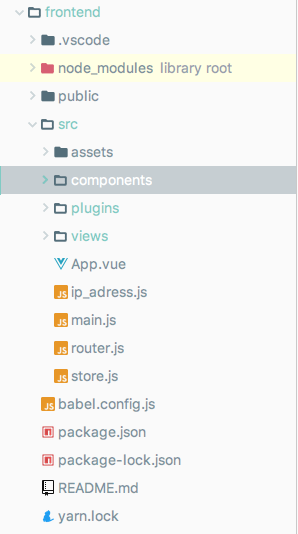
\includegraphics[width=0.3\textwidth]{image/fileTree.png}
    \caption{Файловая структура клиентской части}
    \label{fig:file_tree}
\end{figure}

Типовой файл vue содержит три семантические единицы: 

\begin{itemize}
    \item разметка структуры компонента \mintinline{html}{<template></template>},
    \item программная часть компонента \mintinline{html}{<script></script>},
    \item стили компонента \mintinline{html}{<style></style>}.
\end{itemize}

После написания компонента требуется транспиляция кода в нативный js-код и разметку. 

В качестве сборщика использовался <<Webpack>>. Пример файла компонента представлен на листинге \ref{listing:8}. 

\begin{listing}[H]
   \inputminted[breaklines, breakanywhere, linenos, fontsize=\small]{html}{source/vue_comp.vue}
\caption{Представление главного экрана клиентской части приложения}
\label{listing:8}
\end{listing}

Фреймворк Vuetify предоставляет обширную коллекцию стилизованных компонентов, с возможностью переопределения и доработки. Главный экран приложения представлен на рисунке \ref{fig:main_page}. 
\begin{figure}[H]
    \centering
    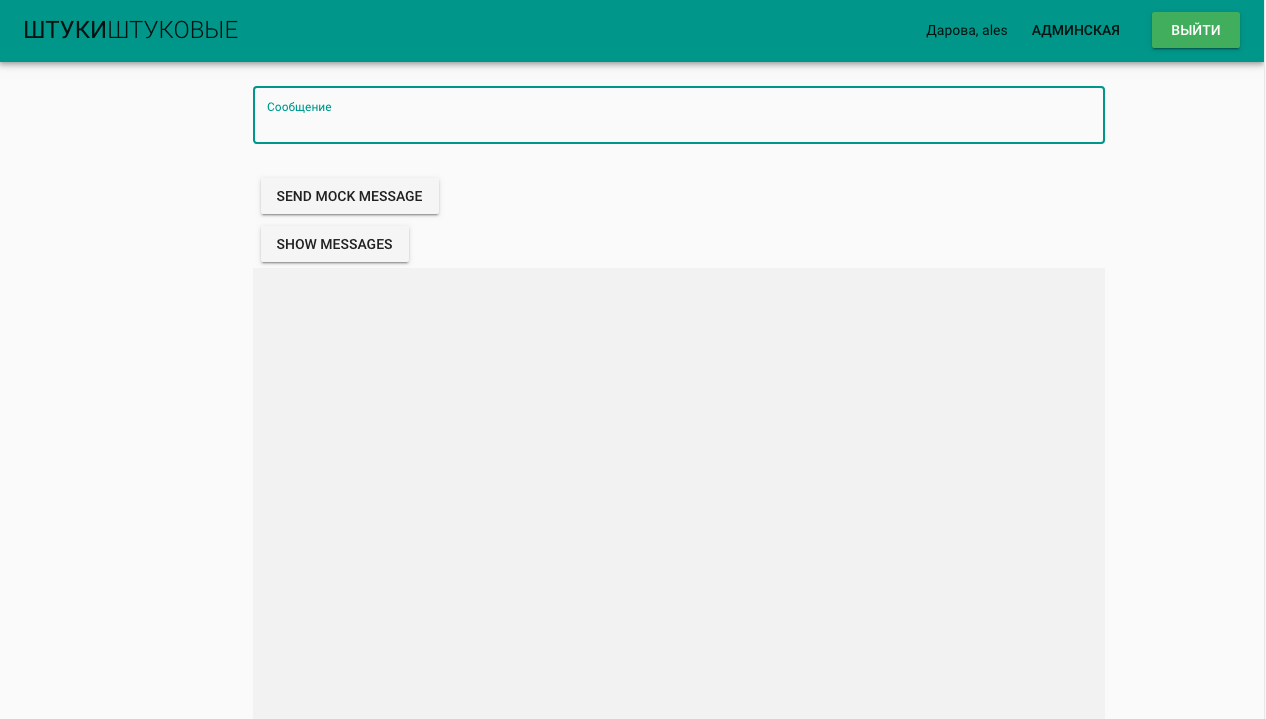
\includegraphics[width=0.9\textwidth]{image/main_page.png}
    \caption{Главная страница приложения}
    \label{fig:main_page}
\end{figure}

На главном экране представлены компоненты чата, переход на страницу администратора и кнопка авторизации. В главном окне пользователь производит общение с чат-ботом. 

При переходе к странице администратора открывается следующая страница представленная на рисунке \ref{fig:admin_page}. 

\begin{figure}
    \centering
    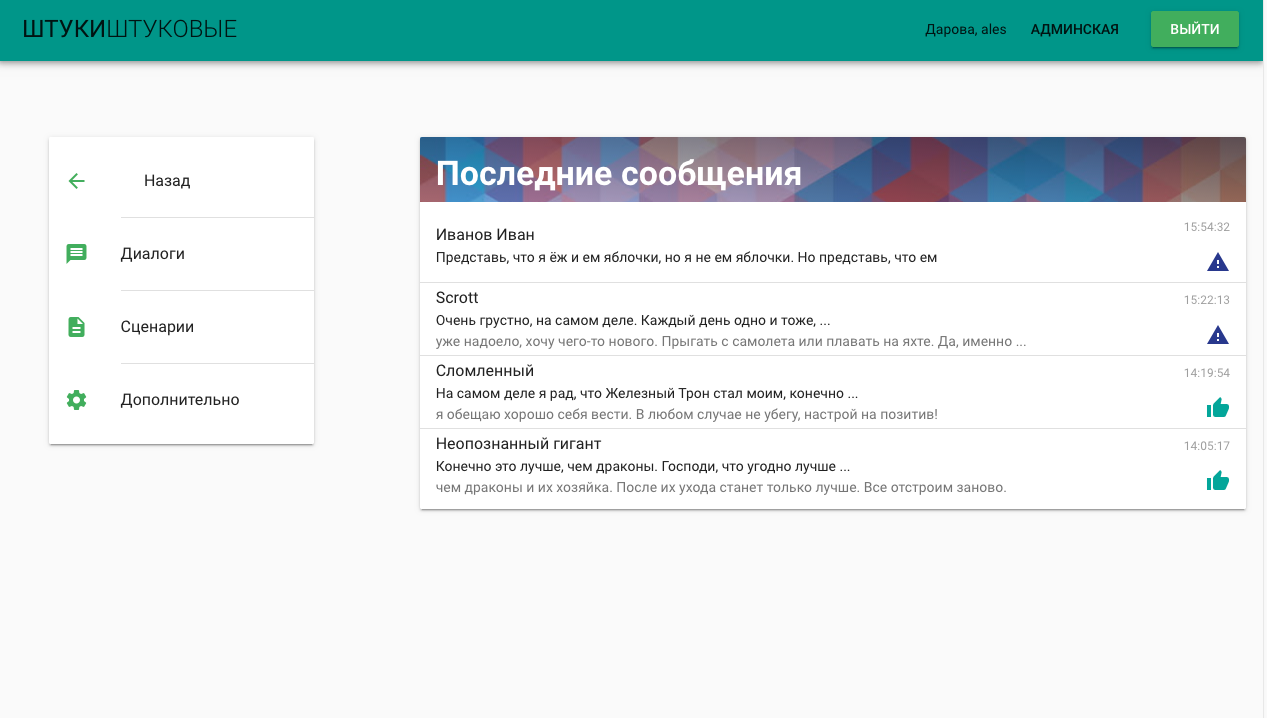
\includegraphics[width=0.9\textwidth]{image/admin_page.png}
    \caption{Страница администратора системы}
    \label{fig:admin_page}
\end{figure}

На страницы расположены вкладки меню, окно отображающее последние сообщения. Каждое сообщение имеет метку времени, заголовок и тело сообщения. Так же сообщение сопровождается меткой анализа тональности. Если сообщение по результатам анализа считается положительным, то используется один тип меток, а если отрицательным, то другой. при нажатии на сообщение происходит переход к телу диалога. 

На рисунке \ref{fig:scenario} представлена страница отображения сценариев. На странице представлен компонент отображающий сценарии бесед в которых бот реагирует на ключевые слова и подбирает реплики из заготовленных сценариев. Если он не находит подходящей реплики, то ответ генерируется при помощи нейросетевой части программы.

\begin{figure}[H]
    \centering
    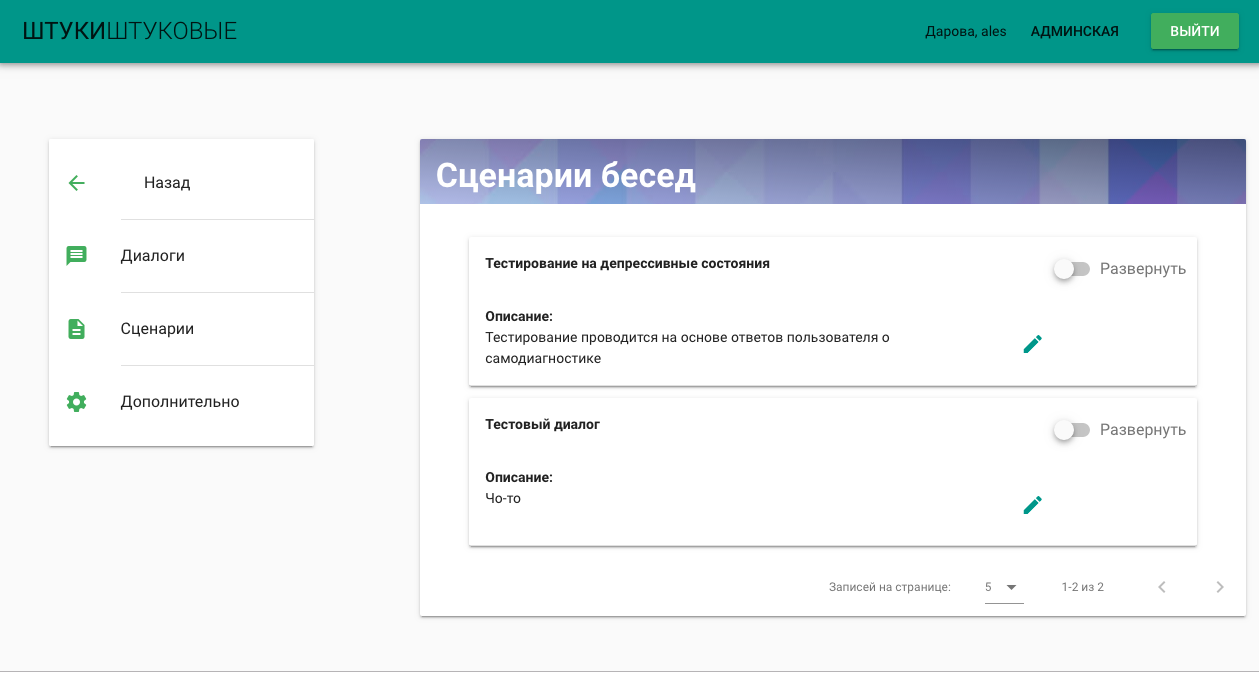
\includegraphics[width=0.9\textwidth]{image/scenario_page.png}
    \caption{Страница сценариев беседы}
    \label{fig:scenario}
\end{figure}

При раскрытии пункта сценария загружаются его компоненты. Пример представлен на рисунке \ref{fig:scenario_open}. При нажатии на реплику осуществляется переход к редактированию сценария. 

\begin{figure}[H]
    \centering
    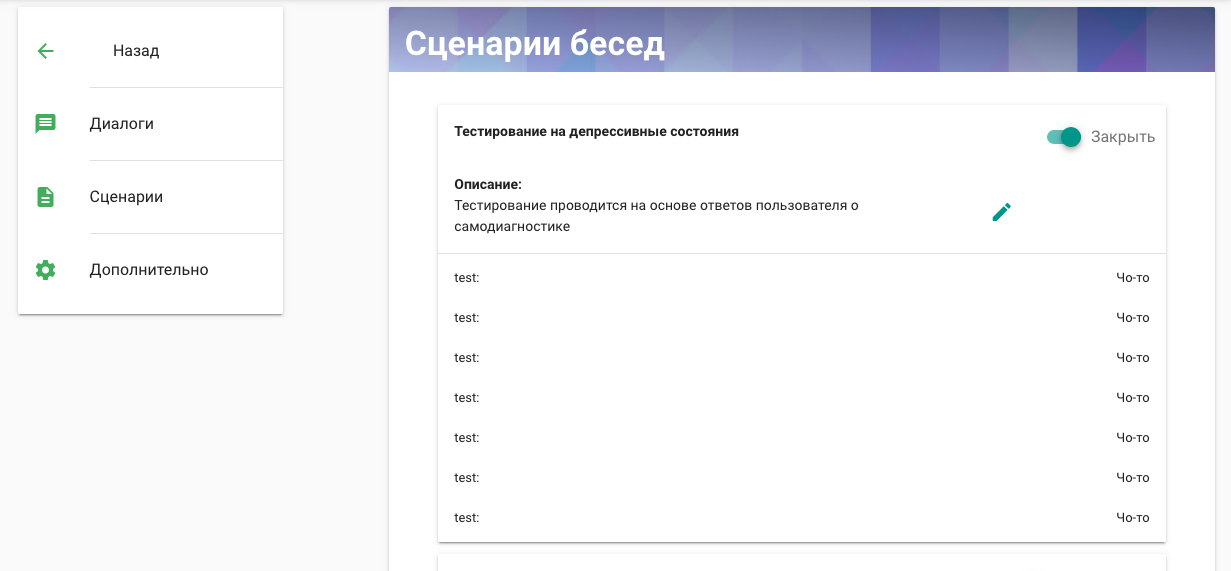
\includegraphics[width=0.9\textwidth]{image/scenario_open_page.png}
    \caption{Пример раскрытия списка реплик сценария}
    \label{fig:scenario_open}
\end{figure}

Пример работы пользователя с программой представлен на рисунках \ref{fig:chat1, fig:chat2}. В них пользователь общается с нейросетевой частью программы, часть поиска шаблонов отключена.   

\begin{figure}[H]
    \centering
    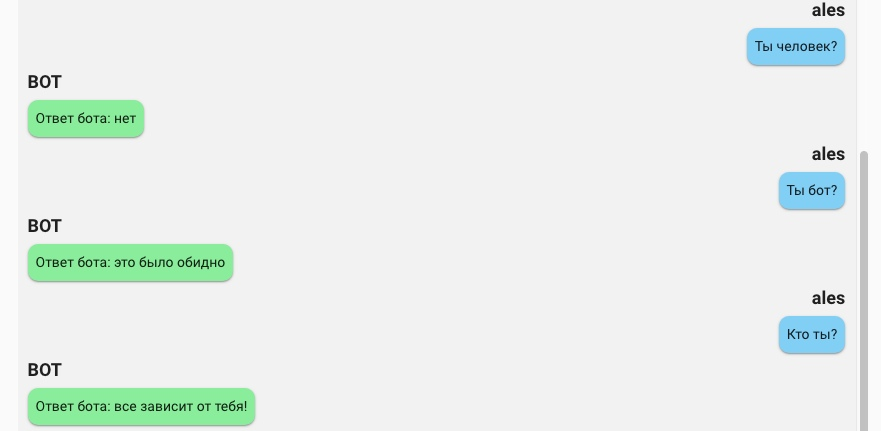
\includegraphics[width=0.9\textwidth]{image/chat.jpg}
    \caption{Пример диалога пользователя}
    \label{fig:chat1}
\end{figure}



\begin{figure}[H]
    \centering
    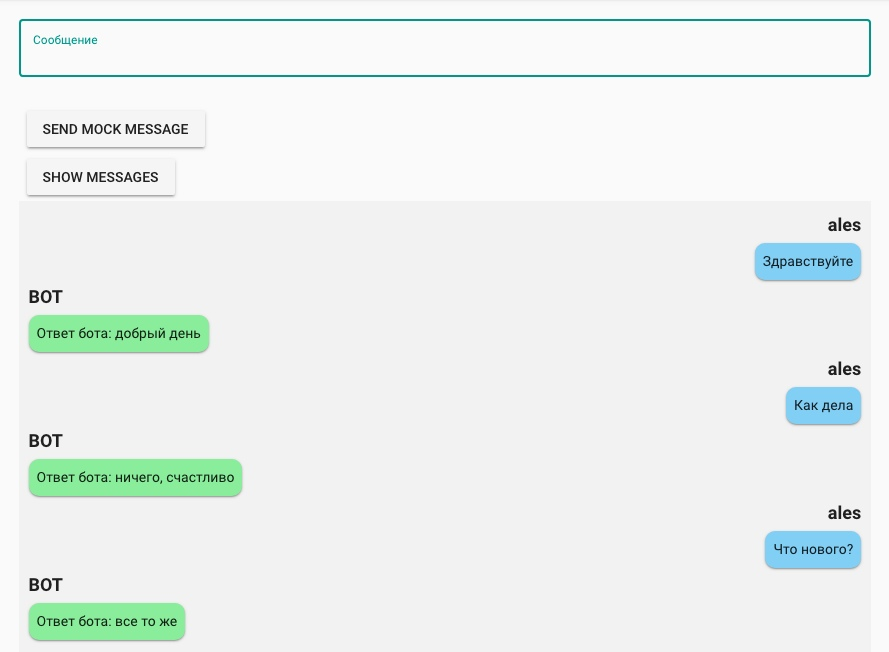
\includegraphics[width=0.9\textwidth]{image/chat2.jpg}
    \caption{Другой пример диалога пользователя}
    \label{fig:chat2}
\end{figure}